\documentclass[svgnames,tikz]{standalone}
\usepackage{pgfmath}
\usetikzlibrary{positioning,arrows,calc,3d}

\tikzset{
  focus/.style args={#1 at #2}{
    insert path={
      %{ [white] (#2.north east) rectangle (#2.south west)}
      ($(#2.center)!#1!(#2.north east) $) rectangle ($(#2.center)!#1!(#2.south west) $)
    }
  },
  focusout/.style args={#1 at #2}{
    even odd rule,
    insert path={
      (#2.north east) rectangle (#2.south west)
      ($(#2.center)!#1!(#2.north east) $) rectangle ($(#2.center)!#1!(#2.south west) $)
    }
  },
  txt/.style={font=\Large\tt},
  img/.style={
     inner sep=2pt,
     draw,
     label/.append style={font=\small\tt},
  },
}


\begin{document}
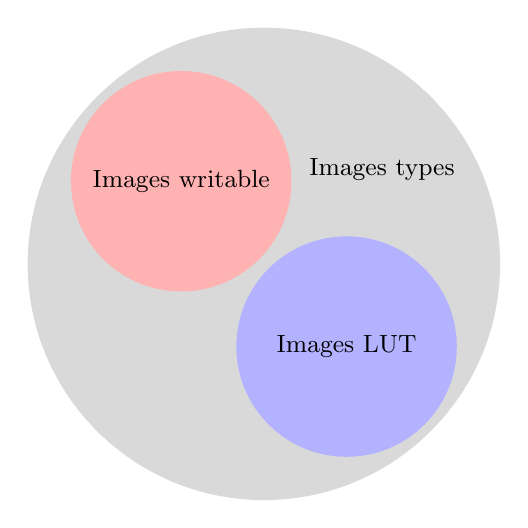
\begin{tikzpicture}
\tikzset{every node/.style={node distance=5pt, font=\small}}

\begin{scope}
  \fill[gray!30!white]  (0, 0)        circle  (3);
  \fill[red!30!white]   (-1.05, 1.05) circle  (1.4);
  \fill[blue!30!white]  (1.05, -1.05) circle  (1.4);
\end{scope}

\node at (1.5, 1.2)     {Images types};
\node at (-1.05, 1.05)  {Images writable};
\node at (1.05, -1.05)  {Images LUT};

\end{tikzpicture}
\end{document}